\section{Results and Discussion}

The practicum was able to identify the internal structure of the models used for machine learning applications, and abstract the content to create a single 32 byte indicator, that can be used as an identifier for uniquely identifying the provenance of machine learning models. The two key applications; recording the changes of the model during the training process locally, and publishing the signature to a cloud repository for verification, validation and traceability all resulted in a mechanism for recording the lifecycle of models.

Beyond looking at simple models, we were able to generate signatures for all default Keras models, as well as sample models used in competitive machine learning challenges. In all cases, we were able to generate a \textit{family tree} of the model's history, as well as an \textit{ancestor} function that identifies the original model used as the baseline for published models. Following the process presented in Figure \ref{fig:lifecycleModels}, we are able to store multiple relationships between models as they are created and published. More importantly, we are not able to remove the model from the global repository.

\begin{figure}[!t]
    \centering
    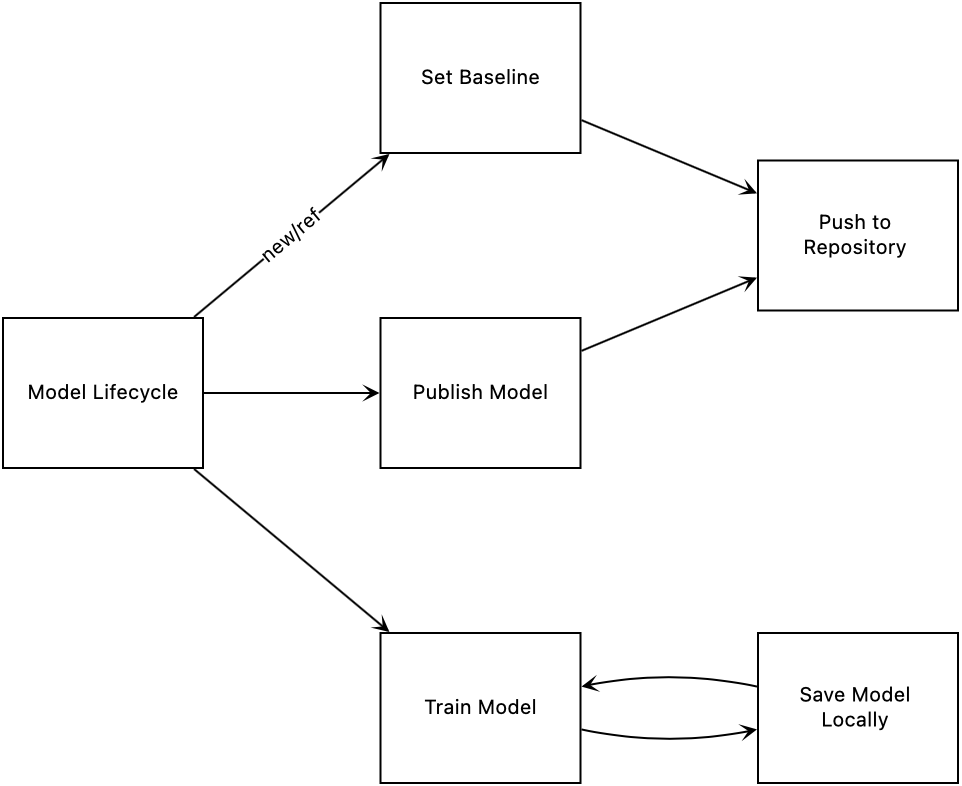
\includegraphics[width=2.5in]{flowchart-4.png}
    \caption{Lifecycle of Software Models}
    \label{fig:lifecycleModels}
\end{figure}

\subsection{Reduction in size for model identification}
The first straightforward result, is being able to produce simplified impressions of models that negate the requirement to store large binary models containing all of the weights, while still providing a utility of being able to determine that a model has changed, how it's structure changes, and which layers have been amended. Below in table \ref{table:memory} is the table of the most common models sizes, which show how much memory is required per iteration, epoch or batch if we wish to retain details of the model. As seen, it shows the high memory cost for some model, which are extracted down to less than one megabyte for the most complex models.

\begin{table}[!ht]
    \centering
    \caption{Memory Usage for Internal Model}
    \label{table:memory}
    \setlength\tabcolsep{0pt} % make LaTeX figure out intercolumn spacing
    \begin{tabular}{@{} p{2cm} p{2cm} p{2cm} p{1cm}  @{}}
        \hline
        Model & Size & Impression Size & Time\\
        \hline
        VGG16       & 528MB & 38.2kb & 4.11s \\
        DenseNet121	& 33MB & 693.8kb & 0.37s \\
        DenseNet169	& 57MB & 952.1kb & 0.53s \\
        Xception	& 88MB & 219.4kb & 0.25s \\
        ResNet50	& 98MB & 292.0kb & 0.41s \\
        ResNet50V2	& 98MB & 311.3kb & 0.42s \\
        MobileNet	& 16MB & 149.3kb & 0.17s \\
        MobileNetV2	& 14MB & 248.5kb & 0.20s \\
        \hline
    \end{tabular}
\end{table}

    Overview of Layers stored in Database
    Comparison of Model Visualisation and Summary

\subsection{Identification of Model History}

One of the most powerful elements for AI practitioners, is the ability to generate a timeline of releases based on when a model is released. In the example shown in figure \ref{fig:lifecycle_in real}, The initial model is shown preserved in both the local and remote repositories. At the end of the model training process, each individual iteration is stored internally with a parent<=>child relationship as part to training process. Once a model is ready for internal testing, it can be baselined, updating the model to point to the original base model. This is shown in the iterations in light blue below. When a model is ready for public release, then the model is baselined.

\begin{figure}[!t]
    \centering
    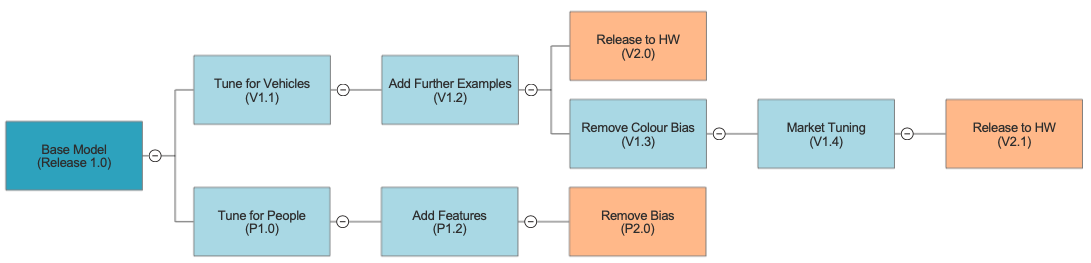
\includegraphics[width=2.5in]{lifecycle.png}
    \caption{Lifecycle of Models in Development Path}
    \label{fig:lifecycle_in real}
\end{figure}

The true power of this is being able to use the system to verify and baseline systems, so they are compliant and can be audited in line emerging standard in AI, such as the EU Artificial Intelligence Act, inspired by the work of the AI HLEG \cite{high-level_expert_group_on_ai_ethics_2019}. Every subsequent model released will be added to the chain, and at anytime the model itself can be used to generate a signature while shows the history.

    Showing the history of the models either locally or remotely
    Identifying the differences between models
    Family Tree of Models

\subsection{Difference between published Models}
    Obtaining an overview of parameter changes of official models

\subsection{Performance}






